\chapter{Resultados}

Os experimentos deste trabalho foram executados em um computador equipado com um processador da Core i7-3770 3.4 GHz da Intel com 4GB de memória RAM e placa de vídeo GeForce GTS 450 com suporte a CUDA (versão 5.0). O teste em vídeo foi feito utilizando diferentes filmagens, com diferentes números de quadros. Todas as filmagens tem resolução de 320 por 240 \emph{pixels} e tiveram como objetivo rastrear um cubo parado enquanto se fazia movimentos com a câmera utilizada na filmagem.

Foram feitos dois tipo de teste: um de performance, que compara o tempo médio para a execução do algoritmo em cada quadro, e o teste de qualidade de rastreamento, que indica, através de um resultado numérico, o quão próxima a pose encontrada está dos pontos extraídos da imagem.

No teste de performance foi medido o tempo, em milésimos de segundos, que o algoritmo leva para executar a etapa de rastreamento (obtenção dos pontos de forte gradiente, escolha das hipóteses, cálculo da pose). Não foi considerado o tempo de obtenção dos quadros a partir da câmera e renderização do modelo na tela do computador, pois isso é bastante dependente dos respectivos \emph{drivers} de entrada e saída. Neste teste será feita uma comparação da velocidade do algoritmo utilizado nesse trabalho (utilizando tanto a implementação em CPU como a implementação em GPU) com o algoritmo de escolha de hipóteses baseado na distância até a amostra do modelo. O ideal é que cada quadro seja computado em pelo menos 33 milésimos de segundo, o que em termos de quantidade de \emph{frames} por segundo é algo em torno de 30 FPS, que é perto do limiar humano de percepção de movimento quadro a quadro.

No teste de qualidade foi utilizado como métrica o erro de reprojeção da pose encontrada após a minimização utilizando o algoritmo de Levenberg-Marquardt. Como foi dito anteriormente, o erro de reprojeção é a média das distâncias de cada hipótese de ponto com sua amostra correspondente do modelo utilizando a pose obtida após a minimização. Os resultados do teste de qualidade são indiferentes à capacidade de processamento da máquina utilizada, portanto também é indiferente se o algoritmo foi executado em GPU ou CPU. Neste teste a qualidade do algoritmo será comparada com uma técnica baseada em arestas com múltiplas hipóteses a qual a hipótese mais próxima da amostra sempre é escolhida.

\section{Teste de qualidade}

No teste de qualidade o principal ponto a se considerar é o erro de reprojeção da pose. Este tipo de métrica é utilizada em outros trabalhos da área \cite{tgchico}.

Os dados mostrados na \figref{qualidade_cubo_real} mostra a variação do erro de reprojeção no decorrer do rastreamento de um cubo. Em determinado momento houve uma movimentação brusca com a câmera após o \emph{frame} 350, onde é possível perceber no gráfico um pico no erro de reprojeção.

\begin{figure}[!ht]
\centering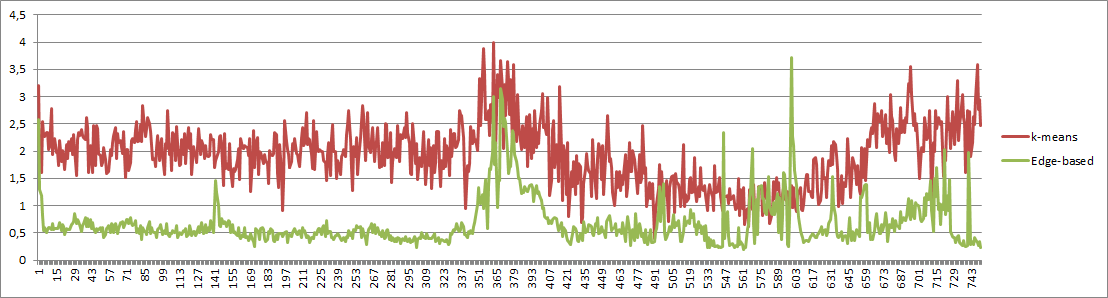
\includegraphics[width=\textwidth]{monografia/qualidade_cubo_real}
\caption{Gráfico de qualidade do rastreamento de um cubo}
\label{qualidade_cubo_real}
\end{figure}

Na \figref{qualidade_cubo_real} é mostrado um gráfico comparativo do rastreamento de múltiplas hipóteses com e sem o algoritmo apresentado neste trabalho. A linha em verde mostra o erro de reprojeção do algoritmo de múltiplas hipóteses tradicional enquanto que a linha vermelha mostra o algoritmo que utiliza a clusterização \emph{k-means}. Foi observado nos testes que apesar das vantagens teóricas para a escolha da melhor hipótese, o técnica discutida apresenta bastante instabilidade na escolha da pose. Mesmo quando a câmera está em repouso, as poses calculadas em dois \emph{frames} consecutivos podem mudar bruscamente. Isso também pode ser observado no gráfico da \figref{qualidade_cubo_real} no que diz respeito à instabilidade no erro de reprojeção da linha vermelha.

Apesar do que foi mostrado no gráfico, ao se analisar o rastreamento quadro a quadro, pode ser visto que em determinado momento (a partir do \emph{frame} 500) o rastreamento utilizando a técnica tradicional de múltiplas hipóteses utiliza uma pose bastante diferente do objeto rastreado, mesmo que o erro de reprojeção continue pequeno. Enquanto que a técnica utilizada neste trabalho apresenta erros de reprojeção maiores, porém a pose se aproxima bastante do objeto. Na \figref{sequencia_cubo_real} é possível observar a sequência de \emph{frames} nos dois casos.

\begin{figure}[!t]
\centering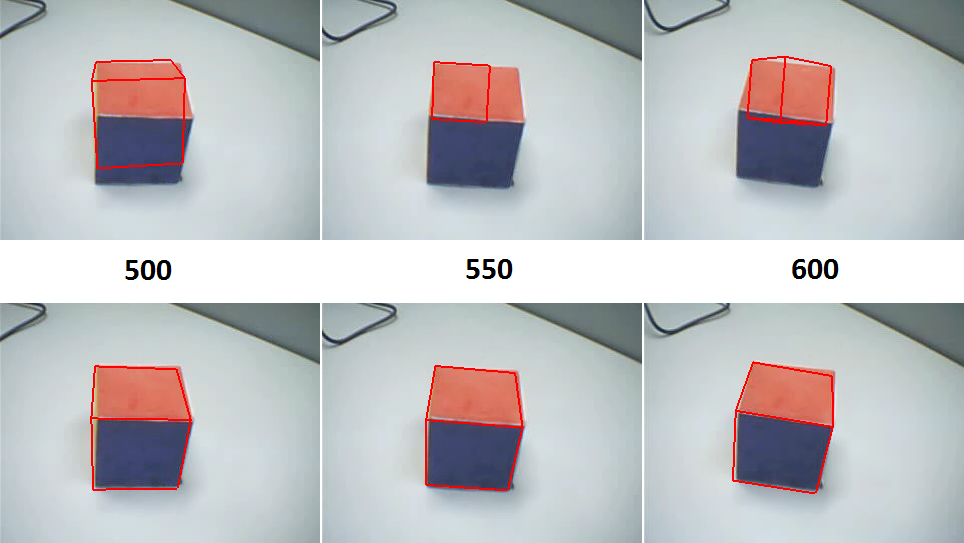
\includegraphics[width=\textwidth]{monografia/sequencia_cubo_real}
\caption{Sequência de imagens comparando as duas técnicas de rastreamento. A imagem mostra tanto o cubo a ser rastreado como também o modelo sendo renderizado. O sequência de baixo é resultado do algoritmo que utiliza múltiplas hipóteses de pose.}
\label{sequencia_cubo_real}
\end{figure}

Foi notado nos experimentos que o algoritmo não apresenta melhora significativa na qualidade de rastreamento comparado com outras técnicas já existentes. O fato das amostras escolhidas serem as mais colineares possíveis torna o rastreamento bastante instável, pois não muito raro as amostras que formam o conjunto mais colinear se distancia bastante da aresta do modelo, chegando em alguns casos uma posição quase que perpendicular a que deveria realmente ser. O algoritmo encontra muita dificuldade em manter a pose escolhida e é possível perceber isso ao analisar o vídeo. Por outro lado notou-se que um ponto forte da técnica é a facilidade em encontrar a pose quando o modelo está bastante distante do real. Nesses casos ele obteve os melhores resultados. No gráfico da \figref{qualidade_celine_boa} pode-se perceber isso. Neste teste, assim como no anterior, um cubo imóvel é rastreado enquanto que a câmera faz todo o movimento, com a diferença que agora são feitos diversos movimentos com a câmera com a intenção de atrapalhar o rastreamento. Com o algoritmo deste trabalho (mostrado em linhas vermelhas), apesar de todas as movimentações, a pose sempre volta ao objeto rastreado, o mesmo não acontece com o algoritmo tradicional.

\begin{figure}[!ht]
\centering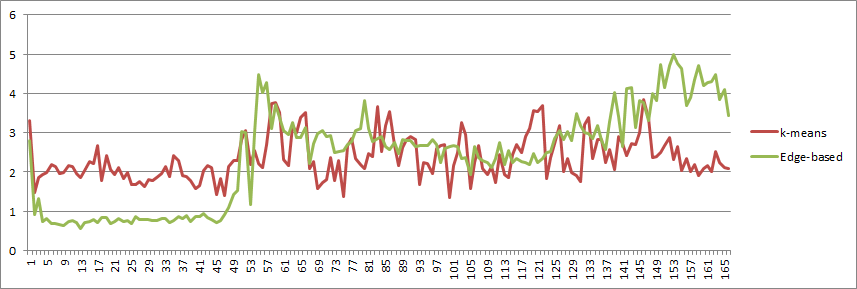
\includegraphics[width=\textwidth]{monografia/qualidade_celine_boa}
\caption{Gráfico comparativo de qualidade em um teste em que são feitos vários movimentos com a câmera}
\label{qualidade_celine_boa}
\end{figure}

\section{Desempenho}

No teste de desempenho é avaliado o tempo, em milésimos de segundo, o qual o algoritmo foi executado. Esse tipo de teste depende bastante da máquina utilizada, mas é importante discuti-lo para se fazer uma comparação relativa entre as técnicas apresentadas. O vídeo de entrada utilizado nos três testes é uma sequência de pouco mais de 700 \emph{frames} de um cubo parado enquanto que a câmera faz alguns movimentos. Foi feito o teste utilizando os algoritmos de múltiplas poses de câmera rodando tanto em GPU quanto em CPU, como também foi utilizado um algoritmo hipótese única de câmera para efeitos de comparação. A \figref{performance} mostra um gráfico comparativo de performance das três simulações. O eixo horizontal mostra os \emph{frames} do vídeo e o eixo vertical mostra o tempo de execução de cada \emph{frame}. Como é um teste de tempo, quanto menor o valor, melhor o resultado. Deseja-se executar o algoritmo em um tempo menor que 33 milésimos de segundo, por cada \emph{frame}, para que a execução seja considerada em tempo real.

\begin{figure}[!ht]
\centering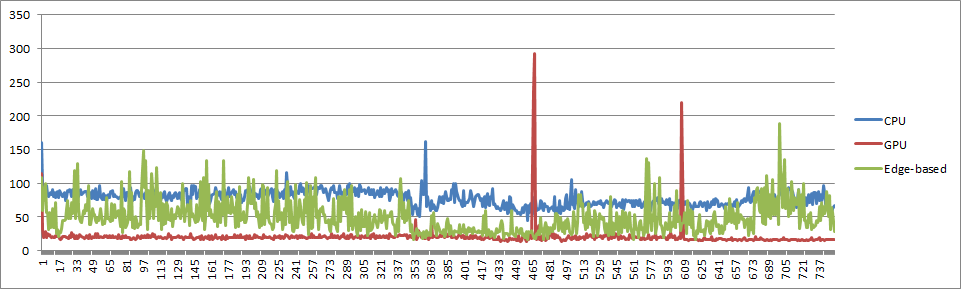
\includegraphics[width=\textwidth]{monografia/performance}
\caption{Gráfico comparativo da performance do algoritmo em CPU e em GPU. Também é mostrado um rastreamento sem utilizar o algoritmo para efeitos de comparação.}
\label{performance}
\end{figure}

A \figref{performance} mostra que o uso de múltiplas hipóteses de pose juntamente com a clusterização \emph{k-means} aumenta bastante o tempo de execução do algoritmo. Apesar disso, o mesmo algoritmo implementado em CUDA apresenta resultados melhores do que a implementação em CPU da técnica de pose única.